\par
Le protocole UDP est utilisé dans les cas suivants :
\begin{itemize}
	\item déconnexion : lorsqu'un joueur souhaite quitter le jeu il envoie une requête de déconnexion au serveur, le serveur reçoit la requête et lui déconnecte du jeu sans lui en informer (sans accusé de réception).
	
	\item envoi du plan de jeu : lorsque le serveur centralise les actions des utilisateurs, il met à jour le plan du jeu et l'envoie aux joueurs; cette opération peut être répétée autant de fois possible sans perturber le jeu.\\
\end{itemize}
Les informations destinées aux joueurs en provenance du serveur, seront envoyées via le broadcast\footnote{Le broadcast permet au serveur d'envoyer un paquet à tous le joueurs connectés}. \\

\par
Le protocole TCP est utilisé à chaque fois qu'il y ait échange entre le serveur et les joueurs sauf dans le cas d'une déconnexion ou d'un envoi du plan de jeu.\\

Les échanges d'informations entre le serveur et les joueurs se feront via des sockets et doivent être fiables, sans erreurs notamment dans le cas d'une connexion d'un joueur au serveur, de la réception par le serveur des actions des joueurs. 
La communication entre le serveur et les joueurs reposent sur des requêtes HTTP. Ci dessous une représentation de cette communication : 

\begin{figure}[ht]
	\centering
	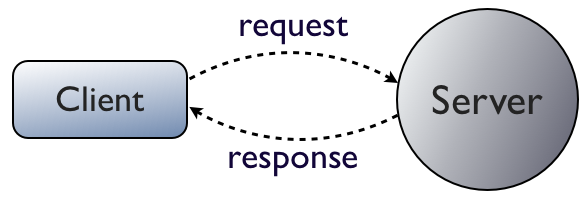
\includegraphics[scale = 0.29]{img/communicationHTTP.png}
	\caption{Communication entre joueur (client) et le serveur}
\end{figure}